\documentclass{article}
\usepackage[utf8]{inputenc}
\usepackage[english]{babel}
\usepackage{amsmath}
\usepackage{natbib}
\usepackage{graphicx}
\usepackage{hyperref}
\usepackage{caption}
\usepackage{caption,float}
\usepackage[vmargin=3cm,hmargin=3cm]{geometry}

\begin{document}

{\centering

\rule{\textwidth}{1.6pt}\vspace*{-\baselineskip}\vspace*{2pt} 
\rule{\textwidth}{0.4pt}\\[\baselineskip] 
{\LARGE Growing Degree Day}
\rule{\textwidth}{0.4pt}\vspace*{-\baselineskip}\vspace{3.2pt}
\rule{\textwidth}{1.6pt}\\[\baselineskip] 

\vspace{20mm} %5mm vertical space
\scshape % Small caps
CMSC 6950 - Computer Based Research Tools and Applications \\ [\baselineskip]
Term Project \\[\baselineskip] 
13th June, 2016 \\[\baselineskip] 
\vspace{20mm} %5mm vertical space
Submitted by \\[\baselineskip]
{\Large Chen Wei \\Thanjida Akhter \\ Md Kamrul Hasan \\ Huizhong Liu \\ Yuan Zhi \par}
\vfill
{\itshape Memorial University of Newfoundland \\ St. John's, Canada.\par} 
}

\newpage

{\centering
  \section*{Abstract}
}

{\itshape In this report, we calculated the growing degree days (GDD) based on different Canadian city's weather history.  The three cities we chose are : St.John's, Halifax, Toronto. \\
}





\section{ \bf Introduction}
Growing degree days (GDD) is simply a predictive tool used in horticulture for accessing crop maturity and development. The equation for calculating the GDD, Eqn.(\ref{eqn:gdd}), is given as follows:

\begin{equation}
\textrm{GDD} = \left(\frac{T_{max} + T_{min}}{2}\right) - T_{base}
\label{eqn:gdd}
\end{equation}

\noindent where {$T_{max}$} is the daily maximum temperature and {$T_{min}$} is the daily minimum temperature. {$T_{base}$} is the base temperature, which is the minimum temperature required for the growth of a particular crop. For the GDD calculations reported in the study, {$T_{base}$} is considered to be 10 $^{\circ}$C.\\


\section{ \bf Data and Graph}
\subsection{Data Collection}
The data for the daily historical temperatures for the selected cities were downloaded from From the collected data, the minimum and maximum daily temperature values all year round were extracted for the selected cities. Daily GDD values were then computed and the results were analyzed and plotted as graphs. A summary of the approach adopted in data collection and analysis is presented below:



\subsection{Growing Degree Day Calculation}
Growing Degree Day (GDD) are calculated by taking the difference between the average daily temperatures and a threshold base temperature, $T_{base}$, (usually 10$^{\circ}$C). The equation for GDD calculation is as follows: \vspace{5mm}

\begin{equation}
\textrm{GDD} = \left(\frac{T_{max} + T_{min}}{2}\right) - T_{base}
\end{equation}

\noindent {$T_{max}$}, {$T_{min}$}, and {$T_{base}$} are the daily maximum, daily minimum and base temperatures, respectively. If the daily mean temperature is lower than the base temperature then $\textrm{GDD} = 0$.In other words, any temperature below $T_{base}$ is set to $T_{base}$ before calculating the average. GDDs are typically measured from the start of spring. A sample GDD calculation for a day in spring with a high of 20$^{\circ}$C and a low of 10$^{\circ}$C is evaluated as follows:\vspace{5mm}

\[ \left(\frac {20+10}{2}\right)-10=5 \] \par

\subsection{ \bf St.Johns }

We analyzed the historical data in 2013 for St.John's. The maximum and minimum daily temperature as figure1 (\ref{1})  




\begin{figure}[H]
\begin{center}
\includegraphics[width=5.25in]{Plot/St.Johns/day_vs_temp_2013.png}

\caption{Cycle of minimum and maximum daily temperatures for St.Johns.}
\label{1}
\end{center}





\end{figure}




\begin{figure}[H]
\centering
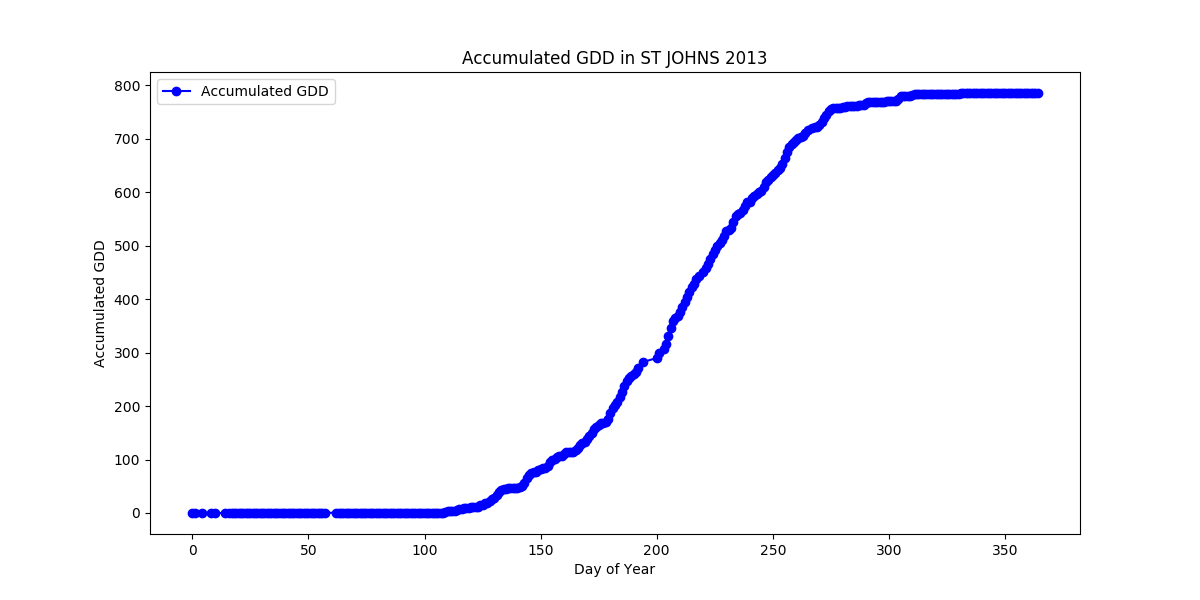
\includegraphics[width=5.25in]{Plot/stjohns.png}



\caption{Accumulated GDD for St.Johns in 2013}
\label{1.1}


\end{figure}



\subsection{ \bf Halifax }

The maximum and minimum daily temperature as figure2 (\ref{2}). From the figure we can conclude that in year 2013, the minimum temperature happened in mid of February 
\begin{enumerate}

\item  Plots 

\begin{center}
\begin{figure}[H]
\includegraphics[width=5.25in]{Plot/HALIFAX/day_vs_temp_2013.png}



\caption{Cycle of minimum and maximum daily temperatures for Halifax}
\label{2}
\end{figure}
\end{center}


\begin{figure}[H]
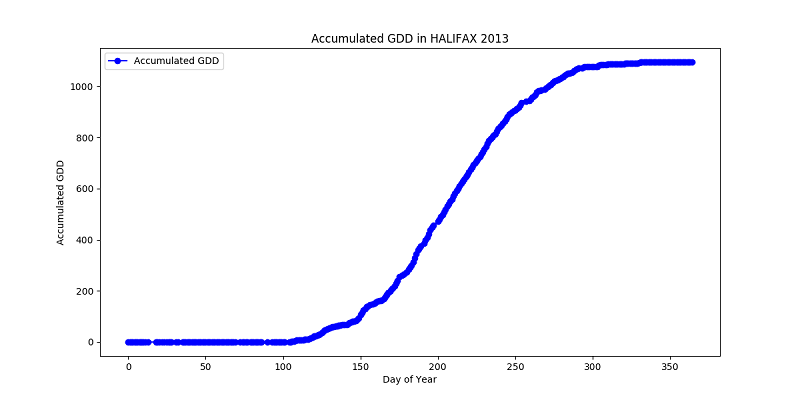
\includegraphics[width=5.25in]{Plot/halifax.png}



\caption{Accumulated GDD for Halifax in 2013}
\label{2.2}
\end{figure}
\end{enumerate}





\subsection{ \bf Toronto }

\begin{enumerate}

\item  Plots 

\begin{center}
\begin{figure}[H]
\includegraphics[width=5.25in]{Plot/Toronto/day_vs_temp_2013.png}



\caption{Cycle of minimum and maximum daily temperatures for Toronto.}
\label{3}
\end{figure}
\end{center}

\begin{figure}[H]
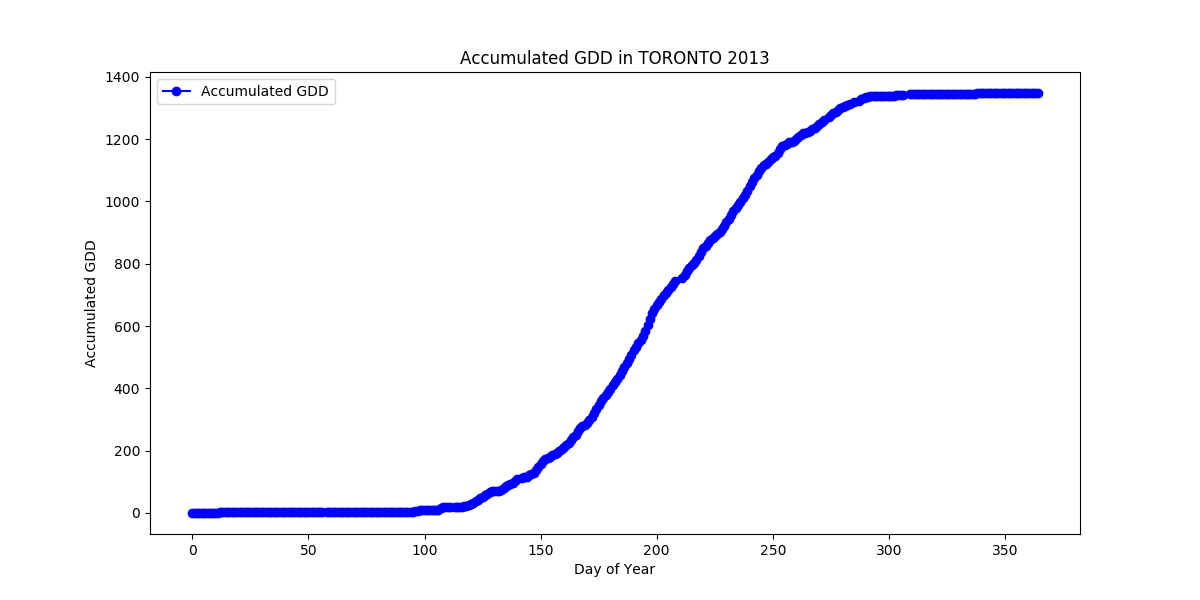
\includegraphics[width=5.25in]{Plot/toronto.png}



\caption{Accumulated GDD for Toronto in 2013}
\label{3.3}
\end{figure}

\end{enumerate}



\subsection{ \bf Vancouver }

\begin{enumerate}

\item  Plots 

\begin{center}
\begin{figure}[H]
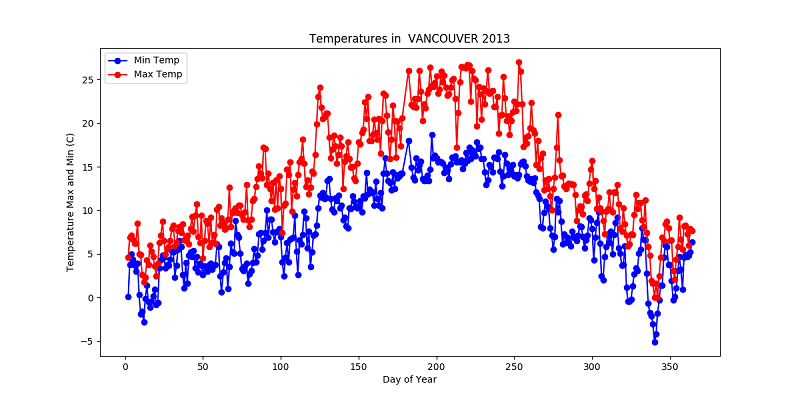
\includegraphics[width=5.25in]{Plot/VANCOUVER/day_vs_temp_2013.png}




\caption{Cycle of minimum and maximum daily temperatures for Vancouver.}
\label{4}
\end{figure}
\end{center}

\begin{figure}[H]
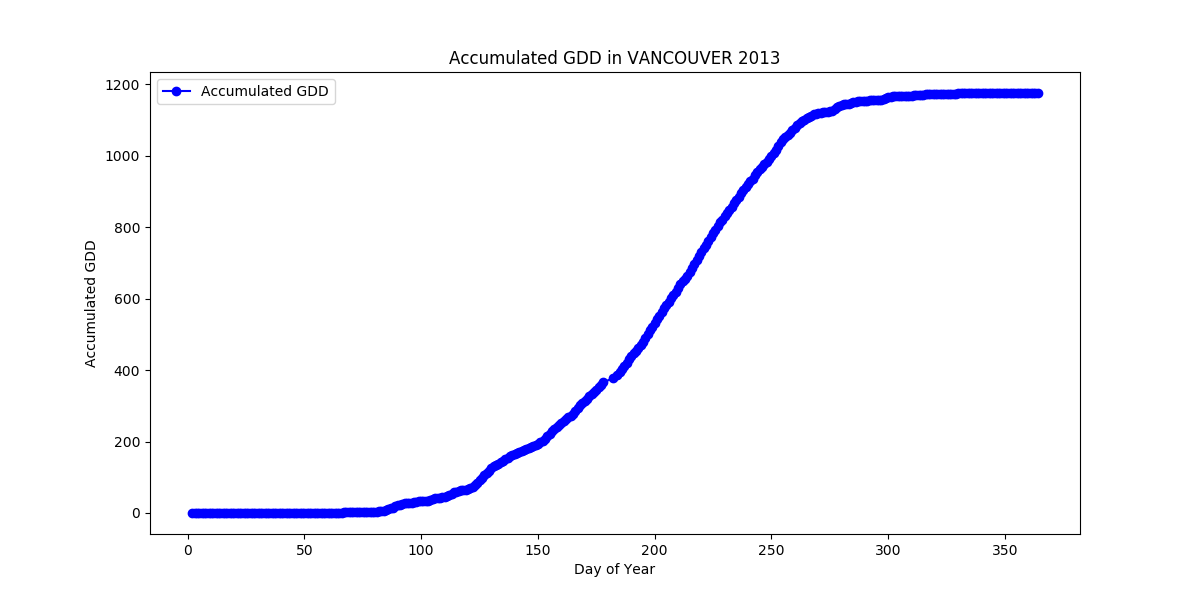
\includegraphics[width=5.25in]{Plot/vancuver.png}



\caption{Accumulated GDD for Vancouver in 2013}
\label{4.4}
\end{figure}

\end{enumerate}







\section{ \bf Results}





\section{Conclusion}


\section{References}
%\bibliographystyle{plain}
\begin{enumerate}
\item Gordon, R.; Bootsma, A. Analyses of growing degree-days for agriculture in Atlantic Canada \textbf{1993} \textit{Clim. Res.} 3: 169--179.
\item \href{url}{$https://en.wikipedia.org/wiki/Growing_degree-day$}
\item \href{url}{$http://www.farmwest.com/node/936$}
\item \href{url}{$http://wine.wsu.edu/research-extension/weather/growing-degree-days/$}
\item \href{url}{$http://whyfiles.org/2010/what-are-growing-degree-days/$}
\end{enumerate}




\end{document}
